\begin{frame}
    \begin{centering}
        \vskip5ex plus 1filll
        {\usebeamerfont{title page title}\usebeamercolor[fg]{title page} Subharmonics\\[1.5ex]}
        \vskip0pt plus 1filll
    \end{centering}
\end{frame}

\begin{frame}{Subharmonics: Motivation}
    Most nonlinear audio effects add higher harmonics to the signal.
    \newline\newline
    What if we want lower harmonics \dots
\end{frame}

\begin{frame}{Subharmonics}
    Goals:
    \vspace{3ex}
    \begin{itemize}
        \item Generate subharmonic content
        \item Avoid circuit modelling
        \item Avoid relying on high-quality pitch detection
    \end{itemize}
\end{frame}

\begin{frame}{Subharmonics}
    Step 1: Detect when the input signal switches directions
    \begin{figure}
        \centering
        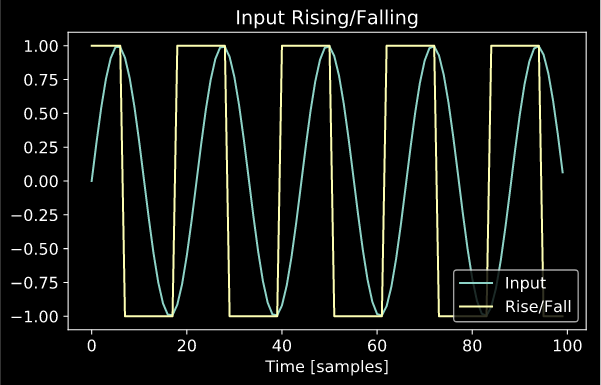
\includegraphics[height=2.5in]{../Subharmonics/Pics/rise_fall.png}
    \end{figure}
\end{frame}

\begin{frame}{Subharmonics}
    Step 2: Flip detector signal every \emph{other} time
    \begin{figure}
        \centering
        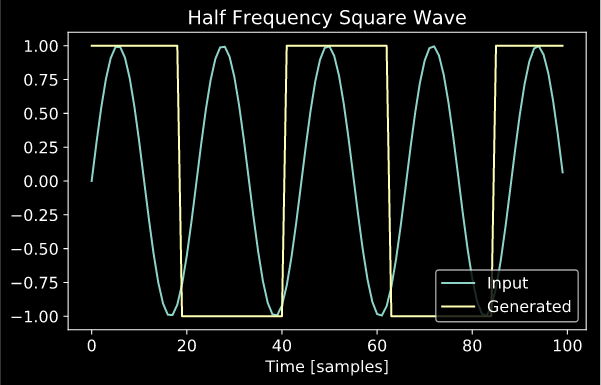
\includegraphics[height=2.25in]{../Subharmonics/Pics/half_square.png}
    \end{figure}
    Result: half-frequency square wave!
\end{frame}

\begin{frame}{Subharmonics}
    Step 3: Lowpass Filter
    \begin{figure}
        \centering
        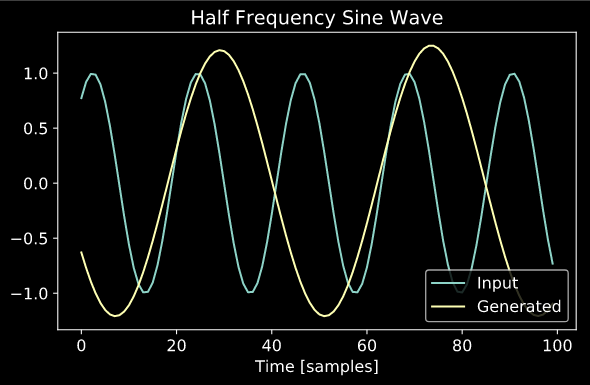
\includegraphics[height=2.5in]{../Subharmonics/Pics/half_sine.png}
    \end{figure}
\end{frame}

\begin{frame}{Subharmonics}
    \begin{figure}
        \centering
        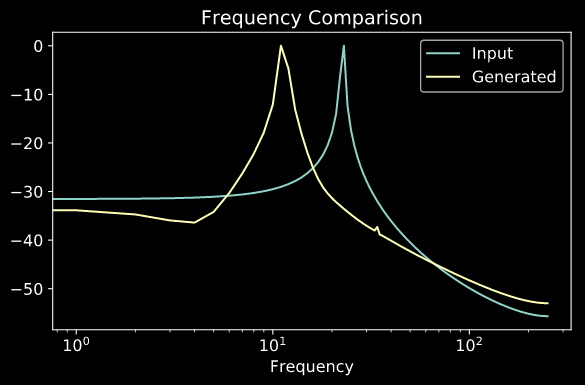
\includegraphics[height=2.5in]{../Subharmonics/Pics/freq_compare.png}
    \end{figure}
\end{frame}

\begin{frame}{Subharmonics}
    Step 4: Apply level detector
    \begin{figure}
        \centering
        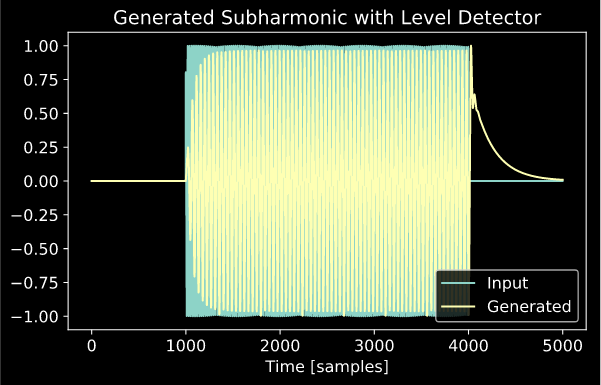
\includegraphics[height=2.5in]{../Subharmonics/Pics/LD_example.png}
    \end{figure}
\end{frame}

\begin{frame}{Subharmonics}
    \begin{figure}
        \centering
        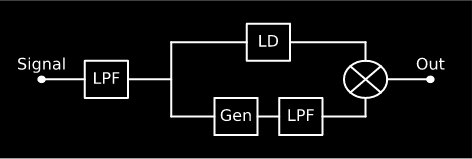
\includegraphics[width=4.5in]{../Subharmonics/Pics/full_arch.png}
    \end{figure}
\end{frame}
